\documentclass[aspectratio=169,11pt]{beamer}
\usepackage[T1]{fontenc}
\usepackage{lmodern,amsmath,amssymb,mathtools,bm,booktabs,array,graphicx,tikz}
\usetikzlibrary{arrows.meta,positioning,calc,decorations.pathreplacing,patterns}
\definecolor{ink}{HTML}{17344D}\definecolor{accent}{HTML}{087E8B}\definecolor{pale}{HTML}{EDF5F5}\definecolor{gold}{HTML}{AD6B19}
\providecommand{\dd}{\,\mathrm{d}}\providecommand{\R}{\mathbb{R}}
\providecommand{\E}{\mathbb{E}}\providecommand{\Var}{\operatorname{Var}}
\providecommand{\Cov}{\operatorname{Cov}}\providecommand{\diag}{\operatorname{diag}}
\providecommand{\norm}[1]{\left\lVert#1\right\rVert}
\providecommand{\abs}[1]{\left|#1\right|}
\usefonttheme{professionalfonts}
\setbeamercolor{normal text}{fg=black,bg=white}
\setbeamercolor{frametitle}{fg=ink,bg=white}
\setbeamercolor{title}{fg=ink}\setbeamercolor{structure}{fg=accent}
\setbeamercolor{block title}{fg=ink,bg=pale}\setbeamercolor{block body}{fg=black,bg=pale!40}
\setbeamercolor{alerted text}{fg=accent}
\setbeamerfont{frametitle}{size=\Large,series=\bfseries}
\setbeamerfont{title}{size=\LARGE,series=\bfseries}
\setbeamertemplate{navigation symbols}{}
\setbeamersize{text margin left=.7cm,text margin right=.7cm}
\setbeamertemplate{frametitle}{\vspace{.18cm}\insertframetitle\par\vspace{.1cm}{\color{accent}\hrule height .6pt}\vspace{.12cm}}
\newcommand{\notestarget}{notes.pdf}\newcommand{\noteslabel}{Notes}
\setbeamertemplate{footline}{\hspace{.7cm}\color{ink}\scriptsize Computational Cardiology\quad\href{\notestarget}{\noteslabel}\hfill\insertframenumber\,/\,\inserttotalframenumber\hspace{.7cm}\vspace{.18cm}}
\setbeamercovered{invisible}
\hypersetup{pdfauthor={Zan Ahmad},pdftitle={A reduced cardiac reaction--diffusion wave},pdfpagemode=UseNone}
\begin{document}
\begin{frame}[plain]\vfill
{\small\color{accent} Computational Cardiology \quad Lecture 10}\par\medskip
{\raggedright\hyphenpenalty=10000\exhyphenpenalty=10000\LARGE\bfseries\color{ink} A reduced cardiac reaction--diffusion wave}\par\bigskip
Zan Ahmad\par\smallskip
{\small Fall 2024}\par\vfill\end{frame}
\renewcommand{\notestarget}{notes.pdf\#note-the-scaled-cardiac-reaction-system}
\begin{frame}[t,fragile,label=slide-a-scaled-cardiac-reaction-system]{A scaled cardiac reaction system}
\[v_t=\frac{hv^2(1-v)}{\tau_{in}}-\frac v{\tau_{out}}+I+Dv_{xx}.\]\pause{} $v,h$ are dimensionless; time is ms and distance is cm.
\end{frame}
\renewcommand{\notestarget}{notes.pdf\#note-the-scaled-cardiac-reaction-system}
\begin{frame}[t,fragile,label=slide-the-recovery-gate]{The recovery gate}
\[h_t=\begin{cases}(1-h)/\tau_{open},&v<v_{gate},\\-h/\tau_{close},&v\ge v_{gate}.\end{cases}\]\pause{} Equality uses the closing branch.
\end{frame}
\renewcommand{\notestarget}{notes.pdf\#note-the-scaled-cardiac-reaction-system}
\begin{frame}[t,fragile,label=slide-the-resting-state]{The resting state}
\[(v,h)=(0,1),\qquad I=0.\]\pause{} Both local derivatives vanish. Homogeneous diffusion also vanishes.
\end{frame}
\renewcommand{\notestarget}{notes.pdf\#note-conservative-coupling-on-a-sealed-strand}
\begin{frame}[t,fragile,label=slide-shared-diffusive-face-fluxes]{Shared diffusive face fluxes}
\[F_{i+1/2}=-D\frac{v_{i+1}-v_i}{\Delta x},\qquad\dot v_i=\frac{F_{i-1/2}-F_{i+1/2}}{\Delta x}.\]\pause{} Sealed endpoints have zero face flux.
\end{frame}
\renewcommand{\notestarget}{notes.pdf\#note-conservative-coupling-on-a-sealed-strand}
\begin{frame}[t,fragile,label=slide-the-chain-laplacian]{The chain Laplacian}
\[\dot v=-L_hv,\qquad L_h\boldsymbol1=0.\]\pause{}\[v^{\mathsf T}L_hv=\frac D{\Delta x^2}\sum_i(v_{i+1}-v_i)^2\ge0.\]
\end{frame}
\renewcommand{\notestarget}{notes.pdf\#note-gate-reaction-and-diffusion-substeps}
\begin{frame}[t,fragile,label=slide-exact-frozen-branch-gate-evolution]{Exact frozen-branch gate evolution}
Below threshold, $h^*=1+(h^n-1)e^{-\Delta t/\tau_{open}}$.\pause{} Above threshold, $h^*=h^ne^{-\Delta t/\tau_{close}}$. Both preserve $[0,1]$.
\end{frame}
\renewcommand{\notestarget}{notes.pdf\#note-gate-reaction-and-diffusion-substeps}
\begin{frame}[t,fragile,label=slide-a-semi-implicit-reaction-step]{A semi-implicit reaction step}
\[a=\frac{h^*(v^n)^2}{\tau_{in}},\qquad v^*=\frac{v^n+\Delta t(a+I)}{1+\Delta t(a+1/\tau_{out})}.\]\pause{} Activation is frozen while the remaining linear factors are implicit.
\end{frame}
\renewcommand{\notestarget}{notes.pdf\#note-gate-reaction-and-diffusion-substeps}
\begin{frame}[t,fragile,label=slide-prove-the-upper-bound]{Prove the upper bound}
\[\text{denominator}-\text{numerator}=1-v^n+\Delta t(1/\tau_{out}-I).\]\pause{} It is nonnegative if $v^n\le1$ and $I\le1/\tau_{out}$.
\end{frame}
\renewcommand{\notestarget}{notes.pdf\#note-gate-reaction-and-diffusion-substeps}
\begin{frame}[t,fragile,label=slide-implicit-diffusion-preserves-the-range]{Implicit diffusion preserves the range}
\[(I+\Delta tL_h)v^{n+1}=v^*.\]\pause{} The inverse is nonnegative and preserves constants, so it maps bounded data into the same interval.
\end{frame}
\renewcommand{\notestarget}{notes.pdf\#note-a-fixed-physical-stimulus-and-sensor-geometry}
\begin{frame}[label=slide-a-fixed-spatial-source-panel-1]{Reduced cardiac front}
\centering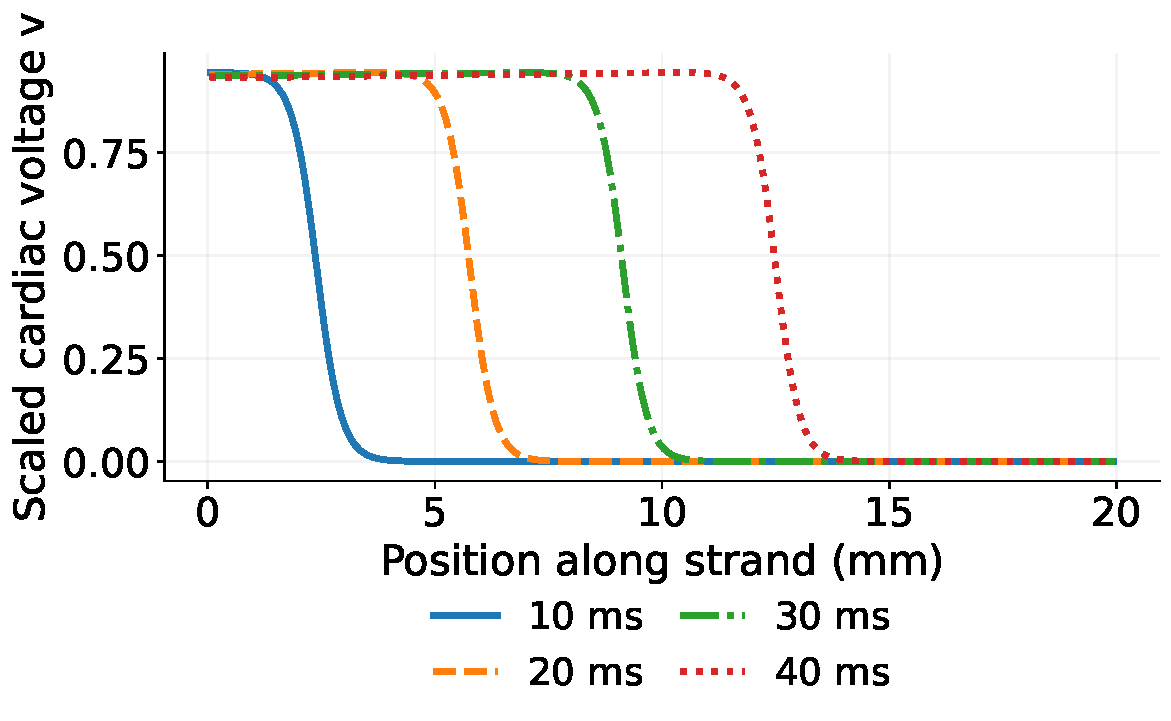
\includegraphics[width=.98\linewidth,height=.69\textheight,keepaspectratio]{presentation-figures/cardiac-wave-panel-1.pdf}\end{frame}
\renewcommand{\notestarget}{notes.pdf\#note-a-fixed-physical-stimulus-and-sensor-geometry}
\begin{frame}[label=slide-a-fixed-spatial-source-panel-2]{Two physical sensors}
\centering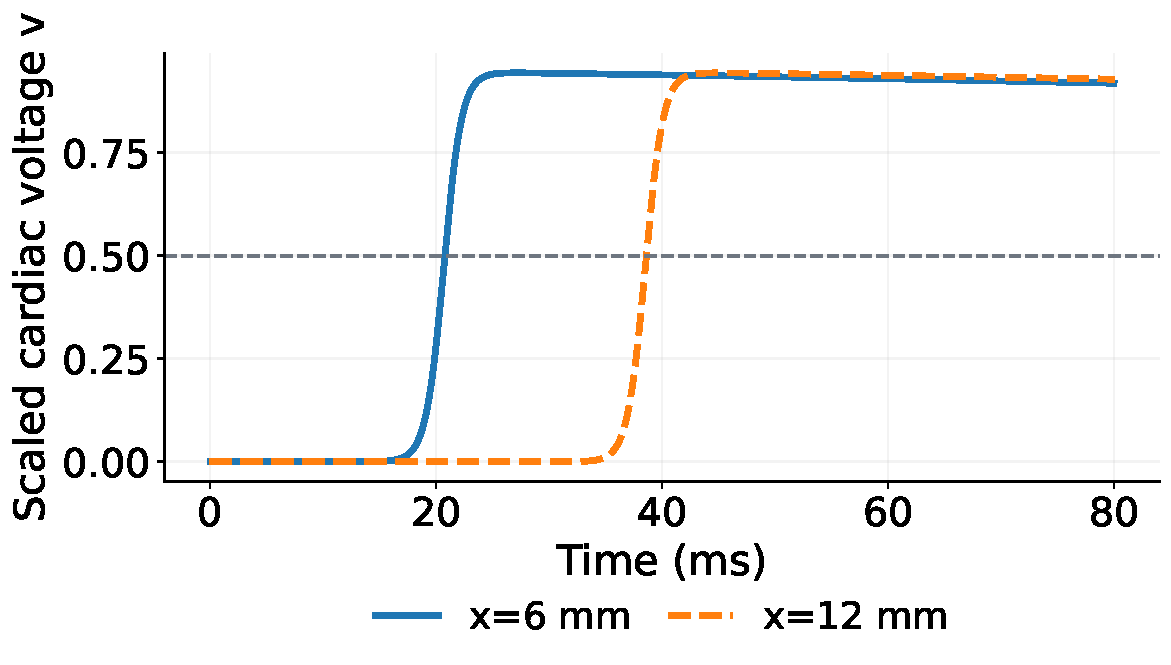
\includegraphics[width=.98\linewidth,height=.69\textheight,keepaspectratio]{presentation-figures/cardiac-wave-panel-2.pdf}\end{frame}
\renewcommand{\notestarget}{notes.pdf\#note-a-fixed-physical-stimulus-and-sensor-geometry}
\begin{frame}[t,fragile,label=slide-a-fixed-spatial-source]{A fixed spatial source}
\[I_i=I_0\frac{|K_i\cap[0,\ell_s]|}{\Delta x}.\]\pause{} Fractional overlap preserves the source width under mesh refinement.
\end{frame}
\renewcommand{\notestarget}{notes.pdf\#note-a-fixed-physical-stimulus-and-sensor-geometry}
\begin{frame}[t,fragile,label=slide-a-fixed-temporal-source]{A fixed temporal source}
\[\int\!\int I\,\mathrm dx\,\mathrm dt=I_0\ell_sT_s=.02\ \mathrm{cm}.\]\pause{} These are scaled-voltage integral units, not microcoulombs.
\end{frame}
\renewcommand{\notestarget}{notes.pdf\#note-threshold-arrival-and-conduction-speed}
\begin{frame}[t,fragile,label=slide-interpolate-an-upward-crossing]{Interpolate an upward crossing}
\[t_*=t_0+\frac{v_*-v_0}{v_1-v_0}(t_1-t_0).\]\pause{} A valid upward bracket and unequal endpoint values are required.
\end{frame}
\renewcommand{\notestarget}{notes.pdf\#note-threshold-arrival-and-conduction-speed}
\begin{frame}[t,fragile,label=slide-define-the-measured-speed]{Define the measured speed}
\[c=\frac{x_2-x_1}{t_{*,2}-t_{*,1}}.\]\pause{} Sensors at $.6$ and $1.2$ cm use the same $v_*=.5$ criterion.
\end{frame}
\renewcommand{\notestarget}{notes.pdf\#note-component-analysis-and-coupled-refinement}
\begin{frame}[label=slide-timing-error-propagates-into-speed-panel-1]{Refine space}
\centering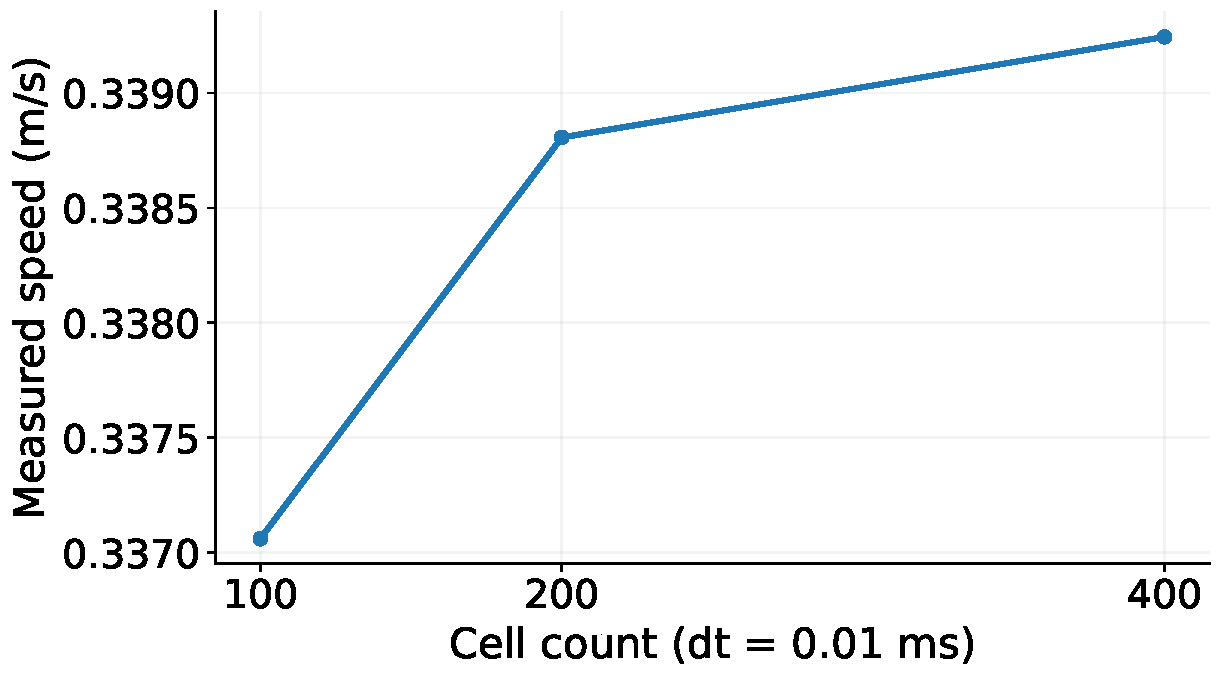
\includegraphics[width=.98\linewidth,height=.69\textheight,keepaspectratio]{presentation-figures/wave-refinement-panel-1.pdf}\end{frame}
\renewcommand{\notestarget}{notes.pdf\#note-component-analysis-and-coupled-refinement}
\begin{frame}[label=slide-timing-error-propagates-into-speed-panel-2]{Refine time}
\centering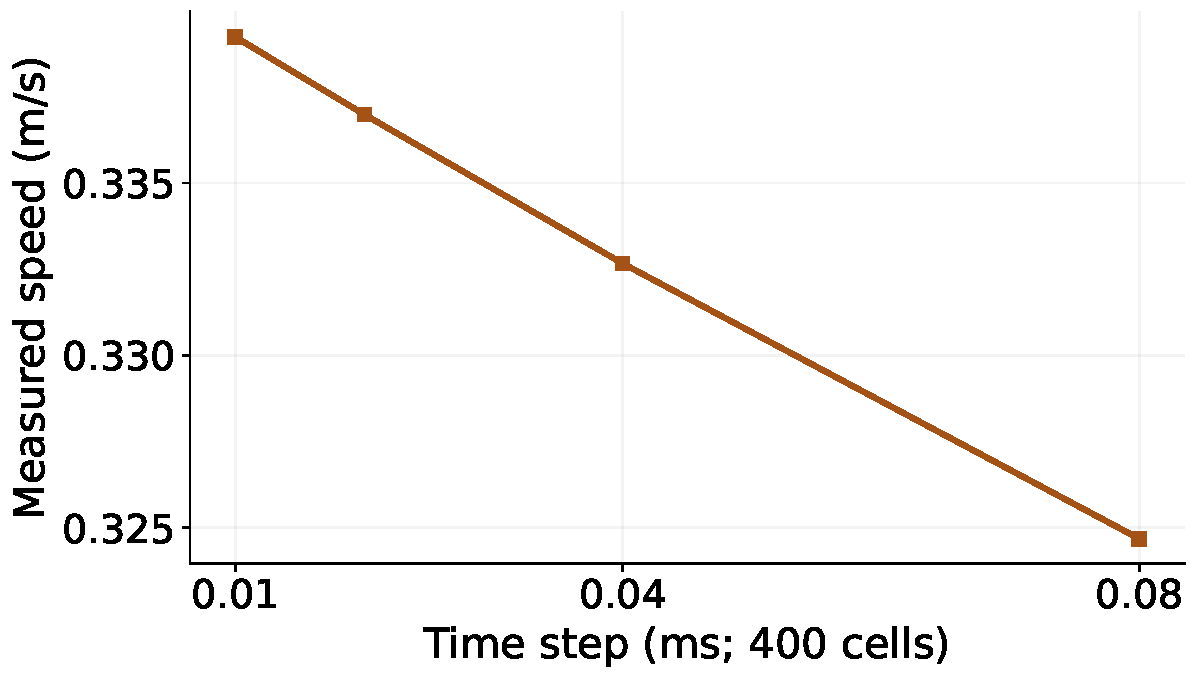
\includegraphics[width=.98\linewidth,height=.69\textheight,keepaspectratio]{presentation-figures/wave-refinement-panel-2.pdf}\end{frame}
\renewcommand{\notestarget}{notes.pdf\#note-component-analysis-and-coupled-refinement}
\begin{frame}[t,fragile,label=slide-timing-error-propagates-into-speed]{Timing error propagates into speed}
\[\frac{\delta c}{c}\simeq-\frac{\delta\Delta t_s}{\Delta t_s}\] for fixed sensor separation.\pause{} Spatial and temporal refinement must retain the same stimulus and sensor definitions.
\end{frame}
\renewcommand{\notestarget}{notes.pdf\#note-component-analysis-and-coupled-refinement}
\begin{frame}[t,fragile,label=slide-scope-of-the-propagation-result]{Scope of the propagation result}
The homogeneous sealed strand omits anisotropy, branching and extracellular potential.\pause{} Bounded states and a plausible speed do not establish a tissue-specific physiological calibration.
\end{frame}
\end{document}
